\chapter{Integration Tests}

\section{Test case scenarios}
\begin{table}[H]
    \begin{tabular}{|l|l|l|p{10cm}|}
    \hline
    Case & Control Unit & Unit under Test & Execution \\ \hline
    1 & CDU & Sensor & CDU sends a get data request to a sensor. \\ \hline
    2 & Sensor & CDU & Sensor sends data to the CDU \\ \hline
    3 & PC & CDU & PC sends a get data request to the CDU \\ \hline
    4 & CDU & Sensor & CDU requests data from a sensor that does not exists \\ \hline
    5 & PC & CDU & PC sends a message to the CDU that the CDU does not recognise. \\ \hline
    6 & Sensor & CDU & Sensor sends invalid data to the CDU \\ \hline
    7 & Sensor & CDU & CDU sends a get data request to a sensor but does not allow the sensor to respond. \\ \hline
    8 & Sensor & CDU & CDU sends a get data request to a sensor. The sensor responds but occupies the bus and never lets go. \\ \hline
    \end{tabular}
\end{table}

\section{Test case results}
\begin{table}[H]
    \begin{tabular}{|l|l|l|p{10cm}|}
    \hline
    Case & Expected result & Actual result & Done \\ \hline
    1 & ~ & ~ & ~\\ \hline
    2 & ~ & ~ & ~\\ \hline
    3 & ~ & ~ & ~\\ \hline
    4 & ~ & ~ & ~\\ \hline
    5 & ~ & ~ & ~\\ \hline
    6 & ~ & ~ & ~\\ \hline
    7 & ~ & ~ & ~\\ \hline
    8 & ~ & ~ & ~\\ \hline
    \end{tabular}
\end{table}

\chapter{Unit Tests}
\section{CDU}
%% The hardware tests of the CDU
This section contains the hardware and software unit tests of the CDU.
\subsection{Hardware}
In order to test the hardware of the CDU, a series of test points was put on the circuitry. External hardware will be needed for some tests. This will be stated clearly if needed.
\subsubsection{Test case 1: 3.3 volt power supply}
\textbf{Purpose:}\\
The purpose of this test is to test the 3.3 volt circuitry of the power supply block in the CDU.\\

\textbf{Procedure:}\\
Apply 20 V on the P+ and P- pins. Measure voltage between 3v3TEST pin and GNDPIN with an oscilloscope.\\

\textbf{Expected Result:}\\
3.35$\pm$0.17 volts are measured.\\

\textbf{Actual Result:}\\
3.36 volts\\

\textbf{Comment and remarks:}\\
Well in range\\

\subsubsection{Test case 2: Communication to bus}
\textbf{Purpose:}\\
The purpose of this test is to test the communication to bus circuitry.\\

\textbf{Procedure:}\\
Apply 20 V on the P+ and P- pins. Between B+ and B- pins put a circuit of 4.7 volt Zener diode and a 5 ohm resistor. Apply 10 kHz signal to INPUTTEST pin. Observe AC coupled signal between SenseTEST pin and GNDPIN with an oscilloscope.\\

\textbf{Expected Result:}\\
10 kHz signal is observed.\\

\textbf{Actual Result:}\\
10 kHz signal is observed.\\

\textbf{Comment and remarks:}\\
-\\

\subsubsection{Test case 3: Voltage reference in receiver circuit}
\textbf{Purpose:}\\
The purpose of this test is to test the voltage reference in receiver circuitry.\\

\textbf{Procedure:}\\
Apply 20 V on the P+ and P- pins. Between B+ and B- pins put a circuit of 4.7 volt Zener diode and a 5 ohm resistor. Measure voltage between REFTEST pin and GNDPIN with an oscilloscope.\\

\textbf{Expected Result:}\\
0.43$\pm$0.02 volts are measured.\\

\textbf{Actual Result:}\\
0.44 volts are measured.\\

\textbf{Comment and remarks:}\\
within range\\

\subsubsection{Test case 4: Communication from bus}
\textbf{Purpose:}\\
The purpose of this test is to test the communication from bus circuitry\\

\textbf{Procedure:}\\
Apply 20 V on the P+ and P- pins. Between B+ and B- pins put a circuit of 4.7 volt Zener diode, a 5 ohm resistor and a BAV21 diode and ZVN3306A. For clarification look at figure ~\ref{fig:busteststub}. Apply 10 kHz signal to the ZVN3306A on the pins shown in the bus test stub figure. Observe AC signal between OUTPUTTEST pin and GNDPIN with an oscilloscope.\\
\begin{figure}[H]
\centering
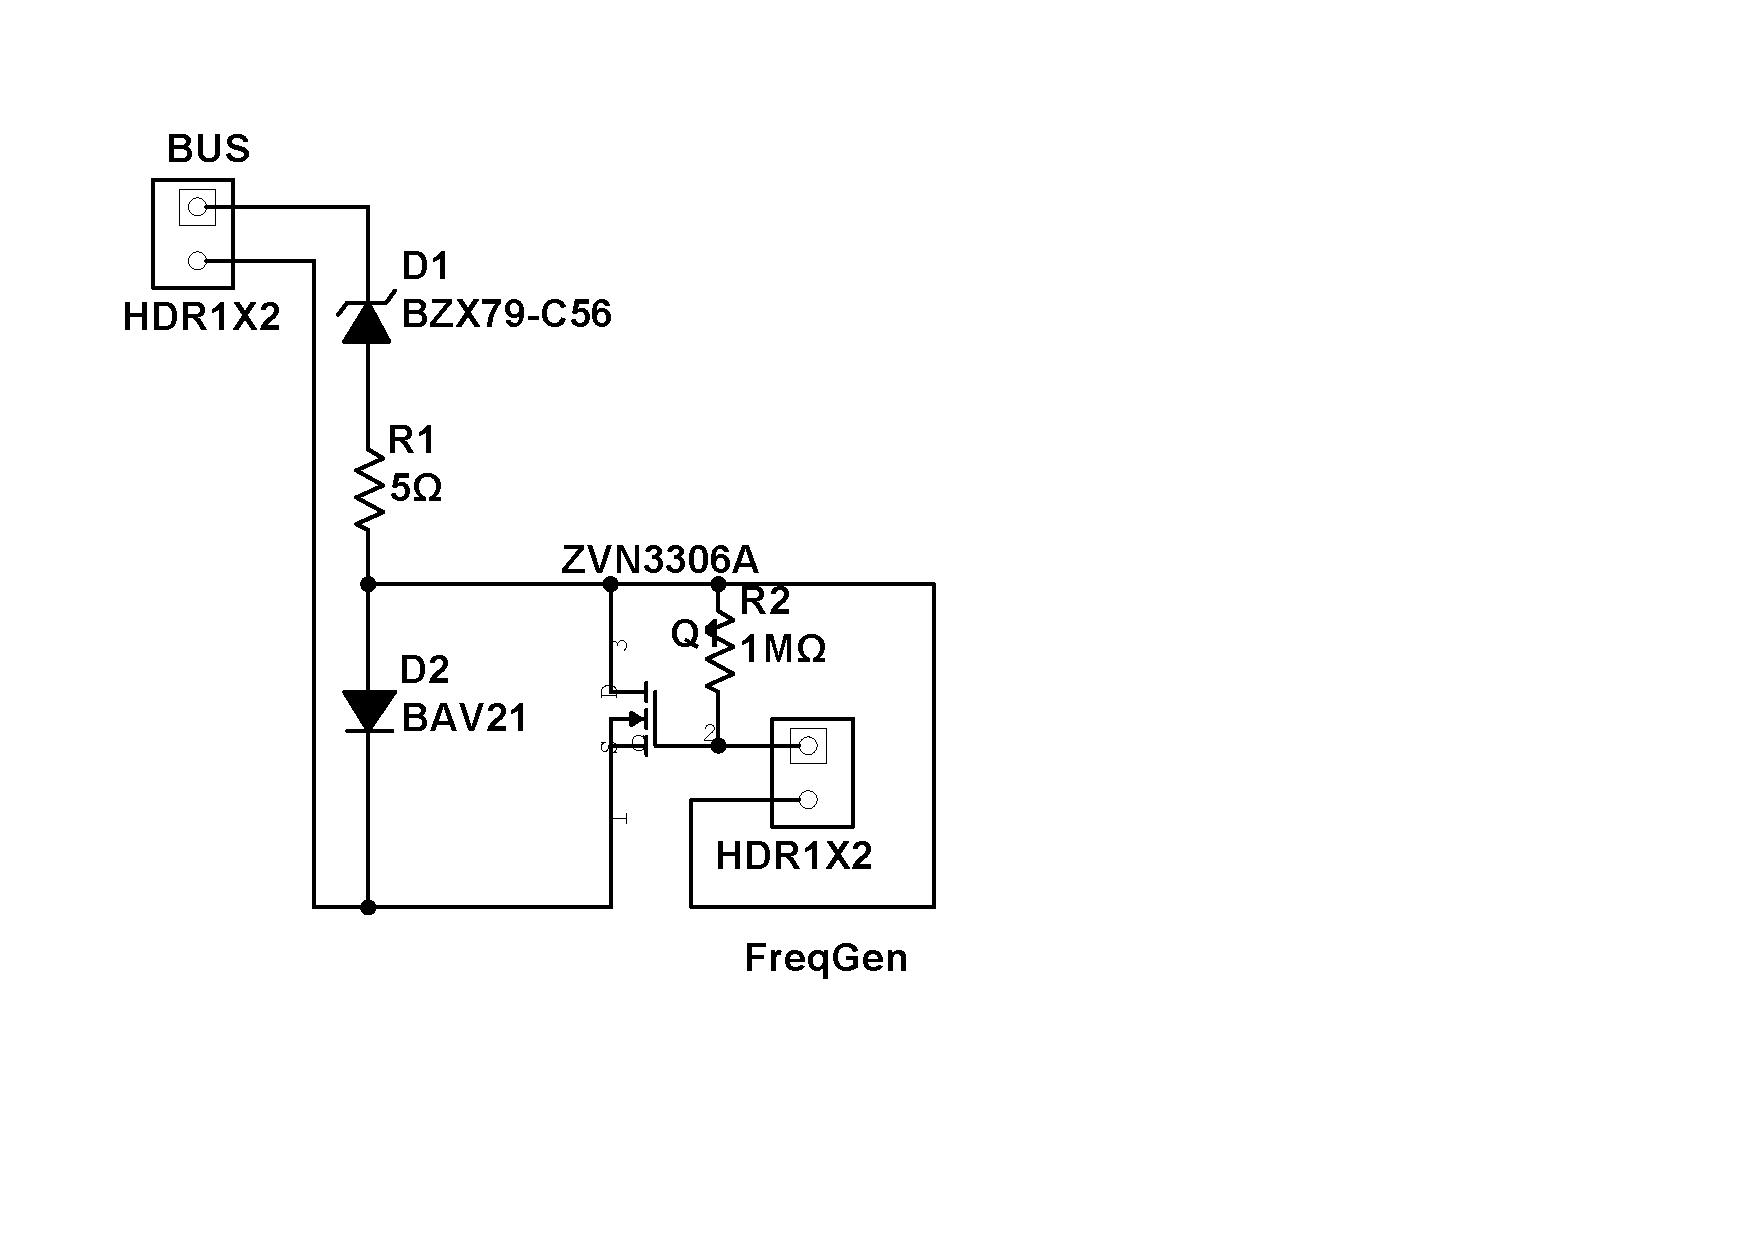
\includegraphics[width=0.8\textwidth]{billeder/BusTestStub}
\caption{Bus test stub}
\label{fig:busteststub}
\end{figure} 


\textbf{Expected Result:}\\
10 kHz signal is observed.\\

\textbf{Actual Result:}\\
\\

\textbf{Comment and remarks:}\\
-\\

\subsection{Software}
The software tests of the CDU

\section{Sensor Node}
\subsection{Hardware}
The hardware tests of the Sensor node
\subsection{Software}
The software tests of the Sensor node